% Preâmbulo comum aos documentos do Grupo VI (classe abnTeX2, normas ABNT).
% Compilar com Tectonic (XeTeX): ver gerar_pdf.sh.
\documentclass[12pt,openright,oneside,a4paper,chapter=TITLE,english,brazil]{abntex2}

% ---------------------------------------------------------------- Fontes
\usepackage{fontspec}
\setmainfont{texgyretermes}[
  Extension=.otf,
  UprightFont=*-regular, BoldFont=*-bold,
  ItalicFont=*-italic, BoldItalicFont=*-bolditalic]
\setmonofont{DejaVuSansMono}[
  Extension=.ttf, BoldFont=*-Bold, Scale=0.82]
\setsansfont{texgyreheros}[
  Extension=.otf,
  UprightFont=*-regular, BoldFont=*-bold,
  ItalicFont=*-italic, BoldItalicFont=*-bolditalic]
\usepackage{amsmath}

% ---------------------------------------------------------------- Pacotes
\usepackage{indentfirst}
\usepackage{graphicx}
\usepackage{xcolor}
\usepackage{booktabs}
\usepackage{array}
\usepackage{tabularx}
\usepackage{longtable}
\usepackage{xltabular}
\usepackage{multirow}
\usepackage[section]{placeins}
\usepackage{enumitem}
\usepackage{listings}
\usepackage{tikz}
\usepackage{adjustbox}
\usetikzlibrary{arrows.meta,positioning,fit,calc,shapes.geometric,backgrounds}
\usepackage[alf,abnt-emphasize=bf]{abntex2cite}

\graphicspath{{../../backend/resultados/}}

% ---------------------------------------------------------------- Aparência
\definecolor{cinzacodigo}{gray}{0.96}
\definecolor{cinzaborda}{gray}{0.75}
\lstset{
  language=Python,
  basicstyle=\ttfamily\small,
  keywordstyle=\bfseries,
  commentstyle=\itshape\color{black!65},
  stringstyle=\color{black!80},
  backgroundcolor=\color{cinzacodigo},
  frame=single, rulecolor=\color{cinzaborda},
  framesep=4pt, xleftmargin=6pt, xrightmargin=6pt,
  columns=fullflexible, keepspaces=true,
  showstringspaces=false, breaklines=true,
  numbers=none, aboveskip=0.8em, belowskip=0.8em,
}
\lstdefinestyle{json}{language={}, basicstyle=\ttfamily\footnotesize, keywordstyle={}}
\renewcommand{\lstlistingname}{Código}
\AtBeginDocument{\renewcommand{\thelstlisting}{\arabic{lstlisting}}}
\renewcommand{\lstlistlistingname}{Lista de códigos}

\setlist{itemsep=0.2em, topsep=0.3em}
\setlist[itemize]{label=--}
\newcolumntype{L}[1]{>{\raggedright\arraybackslash}p{#1}}
\newcolumntype{Y}{>{\raggedright\arraybackslash}X}
\newcolumntype{C}[1]{>{\centering\arraybackslash}p{#1}}
\renewcommand{\arraystretch}{1.25}
\setlength{\arrayrulewidth}{0.5pt}
% Quadros (ABNT): texto, bordas fechadas. Tabelas (IBGE): dados numéricos, laterais abertas.
% Definição do ambiente quadro conforme a documentação do abnTeX2.
\newcommand{\quadroname}{Quadro}
\newcommand{\listofquadrosname}{Lista de quadros}
\newcommand{\quadroautorefname}{Quadro}
\newfloat[chapter]{quadro}{loq}{\quadroname}
\newlistof{listofquadros}{loq}{\listofquadrosname}
\newlistentry{quadro}{loq}{0}
\setfloatadjustment{quadro}{\centering}
\counterwithout{quadro}{chapter}
\renewcommand{\cftquadroname}{\quadroname\space}
\renewcommand*{\cftquadroaftersnum}{\hfill--\hfill}
\setfloatlocations{quadro}{hbtp}

% Fonte de figuras e tabelas produzidas pelo grupo
\newcommand{\fonteautores}{\fonte{Elaborado pelos autores (2026).}}
% Diagrama TikZ: \diagrama{arquivo} reduz a figura à largura do texto, se preciso
\newcommand{\diagrama}[1]{\begin{adjustbox}{max width=\textwidth}\input{figuras/#1}\end{adjustbox}\par}
% Nome de arquivo, função ou campo do código
% (permite quebra de linha depois de \_ e de /)
\newcommand{\codsublinhado}{\textunderscore\allowbreak}
\newcommand{\cod}[1]{{\ttfamily\let\_\codsublinhado#1}}

% ---------------------------------------------------------------- PDF
\makeatletter
\hypersetup{
  pdftitle={\@title},
  pdfauthor={Grupo VI -- Sistemas Distribuídos -- UNIFESSPA},
  pdfsubject={Agregador de Preços de Eletrônicos},
  pdfcreator={LaTeX com abnTeX2},
  colorlinks=false, hidelinks, bookmarksdepth=4}
\makeatother

\setlength{\parindent}{1.25cm}
\setlength{\parskip}{0.2cm}
\setlength{\emergencystretch}{3em}

% Títulos em Times, negrito (seções primárias em caixa alta, como pede a NBR 6024)
\renewcommand{\ABNTEXchapterfont}{\rmfamily\bfseries}
\renewcommand{\ABNTEXchapterfontsize}{\normalsize}
\renewcommand{\ABNTEXsectionfont}{\rmfamily\bfseries}
\renewcommand{\ABNTEXsectionfontsize}{\normalsize}
\renewcommand{\ABNTEXsubsectionfont}{\rmfamily\bfseries}
\renewcommand{\ABNTEXsubsectionfontsize}{\normalsize}
\renewcommand{\ABNTEXsubsubsectionfont}{\rmfamily\itshape}
\renewcommand{\ABNTEXsubsubsectionfontsize}{\normalsize}

% ---------------------------------------------------------------- Capa e folha de rosto
% Versões próprias (NBR 14724): instituição, autores, título, subtítulo, local e ano.
\newcommand{\subtitulodoc}{}
\newcommand{\definirsubtitulo}[1]{\renewcommand{\subtitulodoc}{#1}}
\makeatletter
\newcommand{\capagrupo}{%
  \begin{capa}
    \centering
    {\bfseries\imprimirinstituicao\par}
    \vfill
    {\bfseries\large\MakeUppercase{\imprimirtitulo}\par}
    \ifx\subtitulodoc\@empty\else
      \vspace{0.4cm}{\large\subtitulodoc\par}\fi
    \vfill
    {\imprimirlocal\par}
    {\imprimirdata\par}
    \vspace*{0.5cm}
  \end{capa}}
\newcommand{\folhaderostogrupo}{%
  \begin{folhaderosto}
    \centering
    \vspace*{\fill}
    {\bfseries\large\MakeUppercase{\imprimirtitulo}\par}
    \ifx\subtitulodoc\@empty\else
      \vspace{0.4cm}{\large\subtitulodoc\par}\fi
    \vspace*{\fill}
    \hspace{.45\textwidth}%
    \begin{minipage}{.5\textwidth}
      \SingleSpacing\small
      \imprimirpreambulo
      \par\vspace{0.6cm}
      % nomes na mesma linha, separados por vírgula (\\ de \autor vira ",")
      \textbf{Discentes:} {\def\\{,}\imprimirautor}.\par
      \vspace{0.6cm}
      \textbf{\imprimirorientadorRotulo}~\imprimirorientador
    \end{minipage}\par
    \vspace*{\fill}
    {\imprimirlocal\par}
    {\imprimirdata\par}
    \vspace*{0.5cm}
  \end{folhaderosto}}
\makeatother
\newcommand{\listafiguras}{%
  \pdfbookmark[0]{\listfigurename}{lof}%
  \listoffigures*%
  \cleardoublepage}
\newcommand{\listatabelas}{%
  \pdfbookmark[0]{\listtablename}{lot}%
  \listoftables*%
  \cleardoublepage}
% Página pré-textual com título centralizado e sem número de seção
\newcommand{\paginapretextual}[1]{%
  \pdfbookmark[0]{#1}{\detokenize{#1}}%
  \begin{center}{\ABNTEXchapterfont\MakeUppercase{#1}}\end{center}\vspace{0.8cm}}
\newcommand{\listaquadros}{%
  \pdfbookmark[0]{\listofquadrosname}{loq}%
  \listofquadros*%
  \cleardoublepage}
% Legenda de quadro fora de float (para quadros longos com xltabular)
\newfixedcaption{\legendaquadro}{quadro}
\newcommand{\sumario}{%
  \pdfbookmark[0]{\contentsname}{toc}%
  \tableofcontents*%
  \cleardoublepage}

% Dados da capa e da folha de rosto (comuns aos três documentos).
% Autores na ordem do enunciado (Grupo VI). Para completar os nomes, edite apenas \autor abaixo.
\instituicao{%
  UNIVERSIDADE FEDERAL DO SUL E SUDESTE DO PARÁ -- UNIFESSPA
  \par
  FACULDADE DE SISTEMAS DE INFORMAÇÃO -- FACSI
  \par
  CURSO DE SISTEMAS DE INFORMAÇÃO}
\autor{%
  Youri\\
  José Miguel\\
  Mateus Leitão\\
  Michelangelo\\
  Ângelo}
\orientador[Professor:]{Gleison de Oliveira Medeiros}
\local{Marabá -- PA}
\data{2026}
\newcommand{\naturezatrabalho}{Trabalho~1 da disciplina Sistemas Distribuídos -- Engenharia de Requisitos e Desenvolvimento de um Agregador Concorrente (Tema~6: Agregador de Preços de Eletrônicos), apresentado ao Curso de Sistemas de Informação da Faculdade de Sistemas de Informação da Universidade Federal do Sul e Sudeste do Pará. Grupo~VI.}

\titulo{Agregador Concorrente de Preços de Eletrônicos}
\definirsubtitulo{Relatório Técnico}
\preambulo{\naturezatrabalho}

% Fonte dos gráficos gerados a partir dos experimentos
\newcommand{\fonteexperimentos}{\fonte{Elaborado pelos autores (2026), a partir de \cod{backend/resultados/}.}}

\begin{document}
\selectlanguage{brazil}
\frenchspacing

% ================================================================= PRÉ-TEXTUAIS
\pretextual
\capagrupo
\folhaderostogrupo

% ---------------------------------------------------------------- Resumo
\setlength{\absparsep}{18pt}
\begin{resumo}
Agregadores de preços consultam várias fontes independentes para responder a uma única pesquisa do usuário, e a forma de organizar essas consultas determina o tempo de resposta. Este relatório descreve a implementação e a avaliação experimental de um agregador de preços de eletrônicos em Python, construído apenas com a biblioteca padrão, \textit{sockets} TCP e \textit{multithreading}. O cliente envia a pesquisa a um agregador, que consulta quatro lojas simuladas, cada uma executando como processo servidor independente, de forma sequencial ou concorrente (uma \textit{thread} por loja). As ofertas são consolidadas e ordenadas pelo preço total ou por um índice de custo-benefício, e o sistema trata loja fora do ar, queda durante a consulta, \textit{timeout} e mensagens inválidas sem interromper o serviço. Foram realizados os cinco experimentos do enunciado. Com quatro lojas de 150~ms, o modo sequencial levou 621,1~ms e o concorrente 156,5~ms, um \textit{speedup} de 3,97 vezes, próximo do teórico de quatro. Com latências diferentes, o tempo sequencial acompanhou a soma das latências e o concorrente, a maior delas. O agregador atendeu 50 clientes simultâneos sem falhas, com vazão de 372 requisições por segundo, e entregou resultados parciais corretos em todos os cenários de indisponibilidade. Conclui-se que \textit{threads} são eficazes para consultas independentes limitadas por entrada e saída e que, combinadas com \textit{timeouts}, também limitam o efeito de uma loja lenta ou fora do ar.

\textbf{Palavras-chave}: sistemas distribuídos. sockets TCP. multithreading. agregador de preços. tolerância a falhas.
\end{resumo}

\begin{resumo}[Abstract]
\begin{otherlanguage*}{english}
Price aggregators query several independent sources to answer a single user search, and the way these queries are organized determines the response time. This report describes the implementation and experimental evaluation of an electronics price aggregator written in Python using only the standard library, TCP sockets and multithreading. The client sends a search to an aggregator, which queries four simulated stores, each running as an independent server process, either sequentially or concurrently (one thread per store). Offers are consolidated and ranked by total price or by a cost-benefit index, and the system handles stores that are down, crash during the query, time out or send invalid messages without stopping the service. The five experiments required by the assignment were carried out. With four stores at 150~ms, the sequential mode took 621.1~ms and the concurrent mode 156.5~ms, a speedup of 3.97, close to the theoretical value of four. With different latencies, the sequential time followed the sum of the latencies and the concurrent time followed the largest one. The aggregator served 50 simultaneous clients without failures, with a throughput of 372 requests per second, and returned correct partial results in every unavailability scenario. Threads are effective for independent I/O-bound queries and, combined with timeouts, also bound the effect of a slow or unavailable store.

\vspace{\onelineskip}
\noindent\textbf{Keywords}: distributed systems. TCP sockets. multithreading. price aggregator. fault tolerance.
\end{otherlanguage*}
\end{resumo}

\listafiguras
\listaquadros
\listatabelas
\sumario

% ================================================================= TEXTUAIS
\textual

% =================================================================
\chapter{Introdução}

Comparadores de preço, buscadores de passagens e outros agregadores consultam várias fontes independentes para responder a uma única pergunta do usuário. Cada consulta atravessa a rede e tem latência própria. Por isso, a forma de organizar essas consultas determina o tempo de resposta percebido: uma após a outra (\textbf{sequencial}) ou todas ao mesmo tempo (\textbf{concorrente}) \cite{tanenbaum2007}.

Este trabalho implementa um agregador de preços de eletrônicos baseado em \textbf{sockets TCP} e \textbf{multithreading} em Python \cite{python-socket,python-threading}. O usuário pesquisa um produto (por exemplo, ``rtx 4060'' ou ``notebook'') e o agregador consulta quatro lojas simuladas, cada uma rodando como processo servidor independente. Em seguida, ordena as ofertas pelo preço total (preço + frete) ou por um índice de custo-benefício e destaca a melhor opção. Também foram realizados os cinco experimentos exigidos pelo enunciado \cite{enunciado2026}, que comparam as duas estratégias e avaliam o efeito da latência, a carga de vários clientes e a tolerância à indisponibilidade de uma loja.

O relatório está organizado assim: o \autoref{cap:requisitos} resume os requisitos; o \autoref{cap:modelagem}, a modelagem; o \autoref{cap:implementacao} descreve a implementação; o \autoref{cap:experimentos}, a metodologia dos experimentos; o \autoref{cap:resultados} apresenta e discute os resultados; e o \autoref{cap:conclusao} traz as conclusões. O \autoref{ap:protocolo} traz exemplos das mensagens do protocolo.

% =================================================================
\chapter{Requisitos}\label{cap:requisitos}

A especificação completa está no Documento de Requisitos, organizado como pede a seção~5 do enunciado: descrição do problema, objetivo, escopo, atores, requisitos funcionais e não funcionais, restrições e critérios de aceitação \cite{sommerville2015}. Em resumo:

\begin{itemize}
  \item \textbf{Escopo:} cliente de linha de comando e interface web, agregador TCP, quatro lojas com catálogos simulados, consultas sequenciais e concorrentes, ordenação por preço e custo-benefício, tratamento de falhas, registro de tempos e os cinco experimentos. Ficam de fora lojas e preços reais, autenticação, pagamento, banco de dados e execução entre máquinas.
  \item \textbf{Atores:} Usuário comprador, Pesquisador (experimentos) e Serviço de loja (ator secundário).
  \item \textbf{Interfaces:} o \cod{cliente.py} e a interface web (via gateway HTTP, mais um cliente TCP do agregador) atendem os mesmos requisitos.
  \item \textbf{Restrições:} Python 3.10+ com biblioteca padrão e sockets TCP reais, pelo menos quatro serviços em processos e portas próprios (9001--9004, agregador em 8000), dados simulados em JSON e execução local.
  \item \textbf{Critérios de aceitação:} 18 critérios (CA01--CA18), cada um ligado a um teste automatizado ou a um experimento.
\end{itemize}

Os requisitos funcionais e não funcionais, um para cada exemplo das seções~5.2 e 5.3 do enunciado, estão no \autoref{qua:requisitos}.

\begin{quadro}[!htbp]
  \centering\small
  \caption{Requisitos funcionais e não funcionais}\label{qua:requisitos}
  \begin{tabularx}{\textwidth}{|L{1.4cm}|Y|}
    \hline
    \textbf{ID} & \textbf{Requisito (resumo)} \\ \hline
    RF01 & Informar os parâmetros da pesquisa: produto (com a lista do catálogo), modo e critério. \\ \hline
    RF02 & Consultar pelo menos quatro lojas independentes, cada uma em seu processo. \\ \hline
    RF03 & Permitir consultas sequenciais. \\ \hline
    RF04 & Permitir consultas concorrentes com threads. \\ \hline
    RF05 & Apresentar as ofertas (especificações, frete, garantia, avaliação, tempo por loja) e as lojas sem o produto ou com falha. \\ \hline
    RF06 & Ordenar por preço total ou por custo-benefício. \\ \hline
    RF07 & Identificar o menor preço e o melhor custo-benefício. \\ \hline
    RF08 & Registrar o tempo de execução (total e por loja) e comparar os modos (speedup). \\ \hline
    RNF01 & Comunicação por sockets TCP, com o protocolo JSON documentado. \\ \hline
    RNF02 & Estratégia concorrente com threads (tempo $\approx$ maior latência). \\ \hline
    RNF03 & Atendimento a múltiplas conexões simultâneas ($\geq$ 50 clientes). \\ \hline
    RNF04 & Tratamento de falhas de comunicação sem derrubar o agregador. \\ \hline
    RNF05 & Experimentos de desempenho (latência configurável, execução automatizada). \\ \hline
  \end{tabularx}
  \fonteautores
\end{quadro}

% =================================================================
\chapter{Modelagem}\label{cap:modelagem}

Os diagramas e sua descrição completa estão no documento de Modelagem; esta seção resume os três.

\textbf{Casos de uso (UML).} UC01 Pesquisar produto, UC02 Comparar estratégias, UC03 Listar catálogo, UC04 Executar experimentos e UC05 Usar a interface web (\autoref{fig:casos-uso}). ``Ordenar e identificar melhor oferta'' e ``Registrar tempo de execução'' são incluídos pelo UC01, e ``Tratar falha de loja'' o estende. UC02, UC04 e UC05 incluem o UC01; o UC05 também inclui o UC02.

\begin{figure}[!htbp]
  \centering
  \caption{Diagrama de casos de uso}\label{fig:casos-uso}
  \diagrama{casos_de_uso}
  \fonteautores
\end{figure}

\textbf{Arquitetura.} São três camadas de processos: clientes $\rightarrow$ agregador (porta 8000) $\rightarrow$ quatro lojas (portas 9001--9004), como mostra a \autoref{fig:arquitetura}. Toda a comunicação entre eles usa TCP com mensagens JSON delimitadas por quebra de linha. O navegador fala HTTP apenas com o gateway (porta 8080), que é mais um cliente TCP do agregador.

\begin{figure}[!htbp]
  \centering
  \caption{Diagrama de arquitetura}\label{fig:arquitetura}
  \diagrama{arquitetura}
  \fonteautores
\end{figure}

\textbf{Sequência.} A \autoref{fig:sequencia} mostra a pesquisa em modo concorrente: quatro threads consultam as lojas em paralelo (bloco \textbf{par}), e a falha de uma delas é registrada sem atrasar as demais.

\begin{figure}[!htbp]
  \centering
  \caption{Diagrama de sequência -- pesquisa no modo concorrente, com uma loja fora do ar}\label{fig:sequencia}
  \diagrama{sequencia}
  \fonteautores
\end{figure}

% =================================================================
\chapter{Implementação}\label{cap:implementacao}

\section{Organização do código}

O sistema distribuído fica em \cod{backend/} e a interface web em \cod{frontend/} (\autoref{sec:interface-web}). O \autoref{qua:modulos} descreve os módulos de \cod{backend/}.

\begin{quadro}[!htbp]
  \centering\small
  \caption{Módulos do sistema (\cod{backend/})}\label{qua:modulos}
  \begin{tabularx}{\textwidth}{|L{3.9cm}|Y|}
    \hline
    \textbf{Arquivo} & \textbf{Responsabilidade} \\ \hline
    \cod{protocolo.py} & \textit{Framing} JSON + \cod{\textbackslash n} (\cod{enviar\_json}, \cod{receber\_json}, \cod{requisitar}, \cod{ping}), limite de 64~KB, constantes de operações, modos, critérios e status, exceções \cod{ConexaoEncerrada} e \cod{MensagemInvalida} e validação de pesquisa compartilhada (\cod{validar\_pesquisa}). \\ \hline
    \cod{servidor\_base.py} & \cod{ServidorTCPMultithread}: \cod{accept()} em laço, \textbf{uma thread por conexão}, timeout de ociosidade, respostas de erro padronizadas e proteção contra exceções no tratamento. \\ \hline
    \cod{loja\_server.py} & Serviço de loja: carrega \cod{dados/lojas/<loja>.json}, simula latência (\cod{time.sleep}) e responde \cod{consultar}, \cod{listar\_produtos} e \cod{ping}. \\ \hline
    \cod{agregador.py} & Classe \cod{Agregador}: valida requisições, consulta as lojas (sequencial ou concorrente), consolida, ordena, calcula o custo-benefício e registra o tempo em CSV. \\ \hline
    \cod{cliente.py} & Linha de comando interativa ou por argumentos (\cod{--modo}, \cod{--criterio}, \cod{--atraso}, \cod{--clientes}, \cod{--listar}) com tratamento amigável de erros; \cod{--clientes N} dispara N clientes simultâneos (Exp.~4 ao vivo). \\ \hline
    \cod{config.py} & Endereços, portas, latências e timeouts centralizados. \\ \hline
    \cod{iniciar\_servicos.py} & Sobe as quatro lojas e o agregador como processos e aguarda o \cod{ping} de cada um; no terminal, aceita \cod{derrubar <loja>}, \cod{subir <loja>} e \cod{status} (Exp.~5 ao vivo). \\ \hline
    \cod{experimentos.py}, \cod{graficos.py} & Bateria dos cinco experimentos e geração dos gráficos. \\ \hline
    \cod{gateway\_http.py} & Ponte HTTP/JSON (porta 8080) para a interface web; é um cliente TCP do agregador (\autoref{sec:interface-web}). \\ \hline
    \cod{tests/} & 90 testes automatizados (\cod{unittest}): unidade, integração e sistema. \\ \hline
  \end{tabularx}
  \fonteautores
\end{quadro}

\section{Estratégias de consulta}

O núcleo está em \cod{Agregador.consultar\_todas}, reproduzido no \autoref{cod:consultar-todas}.

\begin{lstlisting}[float=!htbp, caption={Consulta às lojas nos modos sequencial e concorrente (\cod{agregador.py})}, label={cod:consultar-todas}]
def consultar_todas(self, mensagem: dict, modo: str) -> list:
    resultados = [None] * len(self.lojas)

    def tarefa(indice, loja):  # cada thread grava só no seu índice
        resultados[indice] = self.consultar_loja(loja, mensagem)

    if modo == protocolo.MODO_SEQUENCIAL:
        for i, loja in enumerate(self.lojas):
            tarefa(i, loja)                    # espera cada loja responder
    else:
        threads = [threading.Thread(target=tarefa, args=(i, loja))
                   for i, loja in enumerate(self.lojas)]
        for t in threads:
            t.start()                          # dispara as 4 consultas
        for t in threads:
            t.join()                           # aguarda todas
    return resultados
\end{lstlisting}

Cada thread escreve apenas na sua própria posição de uma lista pré-alocada. Por isso não é preciso \textit{lock} para os resultados, e a ordem do cadastro é preservada. O tempo é medido com \cod{time.perf\_counter()} em dois níveis: \cod{tempo\_total\_ms}, da pesquisa inteira, e \cod{tempo\_loja\_ms}, de cada loja. O \textit{speedup} é a razão entre o tempo sequencial e o concorrente:

\begin{equation}
  S = \frac{T_{\text{sequencial}}}{T_{\text{concorrente}}}
\end{equation}

\section{Consolidação e critérios}

O \textbf{preço total} é a soma do preço e do frete, e a ordenação por preço usa esse valor. O índice de \textbf{custo-benefício} (evolução do Tema~6) favorece produtos bem avaliados e com garantia longa, ponderados pelo preço:

\begin{equation}
  \text{score} = \frac{\text{avaliação}^2 \times (1 + 0{,}01 \times \text{garantia\_meses})}{\text{preço\_total}} \times 1000
\end{equation}

A resposta consolidada traz \cod{menor\_preco}, \cod{melhor\_custo\_beneficio}, \cod{ofertas\_ordenadas}, \cod{tempos\_lojas\_ms}, \cod{lojas\_sem\_produto} e \cod{ocorrencias\_ou\_falhas}.

\section{Tratamento de erros e desconexões}

O \autoref{qua:falhas} lista as situações de falha tratadas, como cada uma é detectada e o resultado. Em nenhum caso o agregador é encerrado ou o usuário vê um \textit{traceback}.

\begin{quadro}[!htbp]
  \centering\small
  \caption{Tratamento de erros e desconexões}\label{qua:falhas}
  \begin{tabularx}{\textwidth}{|L{4.3cm}|L{4.4cm}|Y|}
    \hline
    \textbf{Situação} & \textbf{Detecção} & \textbf{Resultado} \\ \hline
    Loja fora do ar & \cod{ConnectionRefusedError} no \cod{connect()} & \cod{erro\_comunicacao} para a loja; a pesquisa continua \\ \hline
    Loja cai durante a consulta & \cod{recv()} retorna vazio $\rightarrow$ \cod{ConexaoEncerrada} & \cod{erro\_comunicacao} imediato, sem esperar o timeout \\ \hline
    Loja travada ou lenta & \cod{socket.timeout} após 2,5~s & \cod{timeout} para a loja \\ \hline
    Mensagem malformada ou maior que 64~KB & \cod{MensagemInvalida} & \cod{erro\_requisicao} \\ \hline
    Loja responde \cod{sucesso} com dados incompletos ou de tipo errado & \cod{validar\_resposta\_loja} $\rightarrow$ \cod{MensagemInvalida} & \cod{erro\_comunicacao} para a loja; a pesquisa continua \\ \hline
    Parâmetro inválido & validação no agregador & \cod{erro\_requisicao} com o motivo \\ \hline
    Cliente conecta e não envia nada & timeout de ociosidade (5~s) & \cod{erro\_requisicao}; a thread é liberada \\ \hline
    Exceção inesperada no servidor & \cod{try}/\cod{except} em \cod{servidor\_base} & \cod{erro\_interno}; o servidor continua no ar \\ \hline
    Agregador fora do ar (no cliente) & \cod{ConnectionRefusedError} & mensagem amigável, código de saída 1 \\ \hline
    Portas já ocupadas ao subir o ambiente & \cod{iniciar\_servicos.porta\_em\_uso} & encerra com código 1, sem deixar processos órfãos \\ \hline
    \cod{iniciar\_servicos.py} recebe Ctrl+C, SIGTERM ou SIGHUP & tratamento de sinais & todas as lojas e o agregador são encerrados \\ \hline
  \end{tabularx}
  \fonteautores
\end{quadro}

\section{Protocolo}

O enunciado pede que o protocolo de aplicação seja documentado com o formato das mensagens, a identificação das operações, o tratamento de erros e o encerramento das conexões \cite{enunciado2026}. A especificação completa está em \cod{docs/03\_protocolo.md}; o \autoref{ap:protocolo} traz exemplos de cada mensagem.

\begin{itemize}
  \item \textbf{Formato das mensagens:} como o TCP entrega um fluxo contínuo de bytes, sem fronteiras entre mensagens \cite{kurose2021}, cada mensagem é um objeto JSON em UTF-8, em uma única linha terminada por \cod{\textbackslash n}. O receptor lê em blocos de 4096 bytes até o \cod{\textbackslash n}; mensagens maiores que 64~KB são recusadas. Toda resposta tem o campo \cod{status}.
  \item \textbf{Identificação das operações:} o campo \cod{operacao} indica \cod{consultar} (pesquisa um produto; aceita \cod{modo}, \cod{criterio} e \cod{atraso\_ms}), \cod{listar\_produtos} (catálogo) ou \cod{ping} (disponibilidade). O mesmo formato é usado nos trechos cliente--agregador e agregador--loja.
  \item \textbf{Tratamento de erros:} seis códigos de status -- \cod{sucesso}, \cod{nao\_encontrado}, \cod{erro\_requisicao}, \cod{erro\_interno}, \cod{erro\_comunicacao} e \cod{timeout}. Os erros têm a forma \cod{\{"status": ..., "detalhe": ...\}}. Falhas de uma loja vão para \cod{ocorrencias\_ou\_falhas} e não invalidam a pesquisa (\autoref{qua:falhas}).
  \item \textbf{Encerramento das conexões:} há uma requisição e uma resposta por conexão. O servidor fecha o socket logo após responder (protocolo sem estado); se o cliente conectar e não enviar nada em 5~s, o servidor responde \cod{erro\_requisicao} e fecha a conexão.
\end{itemize}

\section{Testes}

Os 90 testes automatizados, executados em \cod{backend/} com \cod{python -m unittest discover -s tests}, se dividem em três níveis. Os testes de unidade e de integração sobem lojas e agregador em threads, em portas efêmeras. Os testes de sistema (\cod{tests/test\_sistema.py}) sobem os processos reais nas portas 8000 e 9001--9004 e usam o \cod{cliente.py} como na apresentação. Eles cobrem:

\begin{itemize}
  \item \textit{framing} (fragmentação, JSON inválido, limite de tamanho, conexão encerrada, timeout);
  \item ordenação e menor preço, e equivalência entre os modos sequencial e concorrente;
  \item desempenho (concorrente mais rápido que sequencial; latências heterogêneas);
  \item loja desligada, queda durante a consulta, timeout e todas as lojas fora;
  \item validação de requisições, registro em CSV e 20 clientes simultâneos;
  \item agregador fora do ar no cliente e respostas inválidas de loja (campos ausentes ou de tipo errado);
  \item serviço de loja isolado e gerenciamento de processos (porta ocupada, limpeza, SIGTERM);
  \item roteiro completo da demonstração com processos reais, um passo por experimento;
  \item gateway HTTP da interface web (pesquisa, comparação, validação, falhas, carga, derrubar e subir loja, arquivos servidos).
\end{itemize}

Todos passam. O plano de verificação e testes completo, com a matriz de atendimento ao enunciado, está em \cod{docs/05\_plano\_verificacao\_testes.md}.

\section{Interface web}\label{sec:interface-web}

Para a demonstração há também uma interface web (\cod{frontend/}, Vite + React + TypeScript) com quatro telas: pesquisa e comparação dos modos; lojas e falhas (derrubar e subir cada loja); teste de carga com até 50 clientes simultâneos; e resultados dos experimentos com o registro de pesquisas.

Como o navegador não abre sockets TCP, a interface chama o \textbf{gateway HTTP} (\cod{backend/gateway\_http.py}, só biblioteca padrão: \cod{http.server.ThreadingHTTPServer}). O gateway não substitui nada do sistema: é mais um cliente TCP do agregador e usa a mesma função do \cod{cliente.py}. O HTTP existe apenas entre o navegador e o gateway, e a comunicação agregador--lojas continua igual. Por padrão, o gateway sobe as lojas e o agregador com \cod{iniciar\_servicos.Ambiente}, o que permite derrubar e subir uma loja pela interface; com \cod{--externo}, ele só se conecta a serviços já em execução.

\section{Execução e demonstração}\label{sec:execucao}

O sistema exige apenas Python 3.10+; \cod{matplotlib} é usado só para os gráficos. As instruções completas estão no \cod{README.md} do repositório. Para a demonstração pela linha de comando, em \cod{backend/}:

\begin{itemize}
  \item \textbf{Terminal 1:} \cod{python3 iniciar\_servicos.py} sobe as quatro lojas e o agregador como processos independentes (Ctrl+C encerra tudo). Com o ambiente no ar, esse terminal aceita \cod{derrubar <loja>}, \cod{subir <loja>} e \cod{status}.
  \item \textbf{Terminal 2:} \cod{python3 cliente.py} (interativo) ou \cod{python3 cliente.py rtx 4060}, que roda os dois modos e mostra o \textit{speedup}.
\end{itemize}

O \autoref{qua:roteiro} é o roteiro da demonstração prática, com um passo para cada experimento do enunciado. A interface web (\autoref{sec:interface-web}) é uma alternativa: \cod{python3 backend/gateway\_http.py} e, em \cod{frontend/}, \cod{npm run dev}.

\begin{quadro}[!htbp]
  \centering\small
  \caption{Roteiro da demonstração pelos cinco experimentos}\label{qua:roteiro}
  \begin{tabularx}{\textwidth}{|L{2.8cm}|L{5.9cm}|Y|}
    \hline
    \textbf{Experimento} & \textbf{Comando (terminal 2)} & \textbf{O que mostra} \\ \hline
    1 -- Sequencial & \cod{python3 cliente.py rtx 4060 --modo sequencial} & uma loja após a outra; tempo $\approx$ soma ($\approx$ 600~ms) \\ \hline
    2 -- Concorrente & \cod{python3 cliente.py rtx 4060 --modo concorrente} & uma thread por loja; tempo $\approx$ maior latência ($\approx$ 150~ms) \\ \hline
    3 -- Latência & \cod{python3 cliente.py rtx 4060 --atraso 500} & os dois modos com atraso artificial e o \textit{speedup} \\ \hline
    4 -- Múltiplos clientes & \cod{python3 cliente.py rtx 4060 --clientes 20} & 20 clientes simultâneos em cada modo: tempos, vazão e falhas \\ \hline
    5 -- Indisponibilidade & \cod{python3 cliente.py ssd --modo sequencial --atraso 2000} e, durante a pesquisa, \cod{derrubar MagaluTechSim} no terminal 1 & a pesquisa conclui com 3/4 lojas e o alerta \cod{erro\_comunicacao}; após \cod{subir MagaluTechSim}, volta a 4/4 \\ \hline
  \end{tabularx}
  \fonteautores
\end{quadro}

% =================================================================
\chapter{Experimentos}\label{cap:experimentos}

Os cinco experimentos seguem a seção~9 do enunciado \cite{enunciado2026}. Esta seção descreve o ambiente e a metodologia; os resultados estão no \autoref{cap:resultados}.

\begin{itemize}
  \item \textbf{Ambiente:} macOS (Darwin arm64), 10 CPUs, Python 3.15.0, tudo em \cod{127.0.0.1}.
  \item \textbf{Execução de referência:} bateria completa de 14/11/2026 (14h03), com a versão final do código. A saída completa está em \cod{backend/resultados/saida\_experimentos.txt}.
  \item \textbf{Processos:} quatro lojas e o agregador como processos independentes (\cod{iniciar\_servicos.Ambiente}). As medições passam pelo cliente TCP real.
  \item \textbf{Latência simulada:} \cod{time.sleep} na loja antes de responder, representando o tempo de rede e de processamento de um serviço remoto. A latência vem do campo \cod{atraso\_ms} da requisição ou da configuração de cada loja.
  \item \textbf{Métrica principal:} \cod{tempo\_total\_ms} medido no agregador. No Exp.~4 também foi medido o tempo de resposta no cliente.
  \item \textbf{Repetições:} 30 por modo (Exp.~1 e 2); 10 por ponto (Exp.~3); 3 rodadas por ponto (Exp.~4). As tabelas mostram média, desvio-padrão, mínimo e máximo.
  \item \textbf{Produto pesquisado:} ``notebook'' (as quatro lojas o possuem).
  \item \textbf{Reprodução:} em \cod{backend/}, executar \cod{python experimentos.py} e depois \cod{python graficos.py}. Os dados brutos ficam em \cod{resultados/*.csv} e as tabelas em \cod{resultados/tabelas.md}.
\end{itemize}

O \autoref{qua:experimentos} resume a configuração de cada experimento.

\begin{quadro}[!htbp]
  \centering\small
  \caption{Configuração dos experimentos}\label{qua:experimentos}
  \begin{tabularx}{\textwidth}{|L{4.4cm}|Y|}
    \hline
    \textbf{Experimento} & \textbf{Configuração} \\ \hline
    1 -- Sequencial & 4 lojas × 150~ms, modo sequencial, 30 repetições \\ \hline
    2 -- Concorrente & 4 lojas × 150~ms, modo concorrente, 30 repetições \\ \hline
    3a -- Latência uniforme & 0, 50, 100, 200, 350 e 500~ms em todas as lojas \\ \hline
    3b -- Latência heterogênea & lojas com 100, 200, 300 e 400~ms \\ \hline
    4 -- Múltiplos clientes & 1, 5, 10, 20 e 50 clientes disparados juntos (barreira), lojas com 100~ms \\ \hline
    5 -- Indisponibilidade & MagaluTechSim: (a) desligada antes; (b) derrubada durante a consulta; (c) lenta além do timeout; (d) recuperada \\ \hline
  \end{tabularx}
  \fonteautores
\end{quadro}

% =================================================================
\chapter{Resultados}\label{cap:resultados}

\section{Experimentos 1 e 2 -- sequencial × concorrente}

A \autoref{tab:exp12} e a \autoref{fig:g1} comparam as duas estratégias com quatro lojas de 150~ms.

\begin{table}[!htbp]
  \centering\small
  \caption{Tempo total da pesquisa -- 4 lojas de 150~ms}\label{tab:exp12}
  \begin{tabular}{@{}lrrrrrr@{}}
    \toprule
    \textbf{Modo} & \textbf{n} & \textbf{Média (ms)} & \textbf{Desvio (ms)} & \textbf{Mín. (ms)} & \textbf{Máx. (ms)} & \textbf{Speedup} \\
    \midrule
    Sequencial  & 30 & 621,11 & 2,52 & 612,83 & 623,64 & 1,00 \\
    Concorrente & 30 & 156,50 & 0,24 & 156,01 & 156,89 & \textbf{3,97} \\
    \bottomrule
  \end{tabular}
  \fonteexperimentos
\end{table}

\begin{figure}[!htbp]
  \centering
  \caption{Tempo total: sequencial × concorrente (Exp.~1 e 2)}\label{fig:g1}
  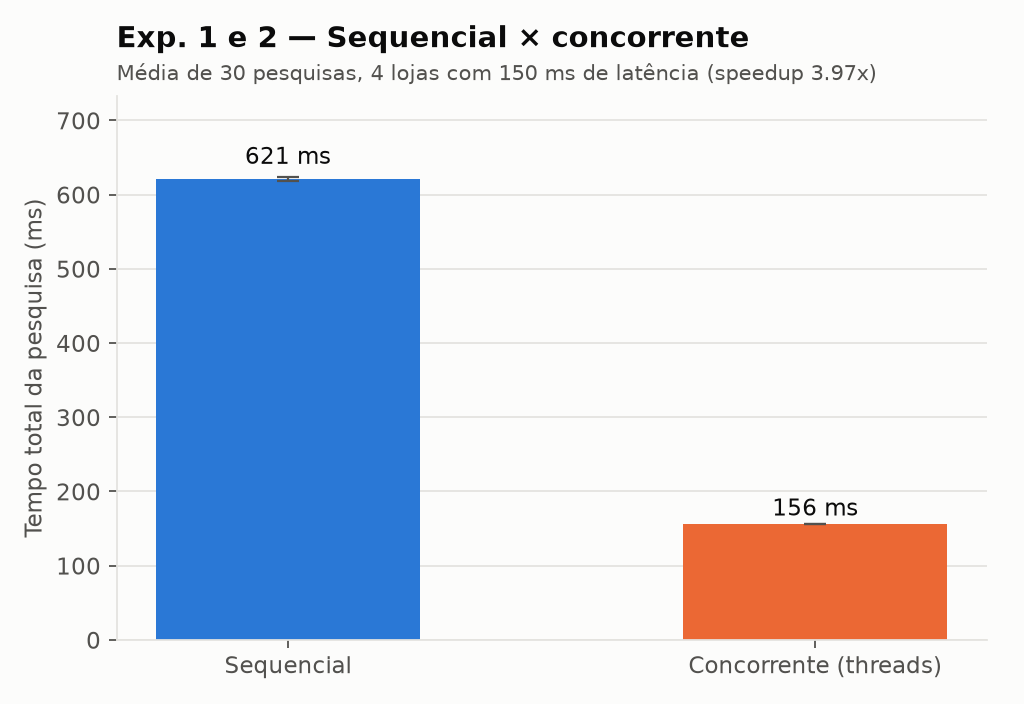
\includegraphics[width=0.78\textwidth]{g1_sequencial_vs_concorrente.png}
  \fonteexperimentos
\end{figure}

\section{Experimento 3 -- simulação de latência}

\subsection{Latência igual em todas as lojas (3a)}

Na \autoref{tab:exp3a} e na \autoref{fig:g2}, a mesma latência artificial é aplicada às quatro lojas, de 0 a 500~ms.

\begin{table}[!htbp]
  \centering\small
  \caption{Tempo médio por latência artificial, igual nas quatro lojas (10 repetições por ponto)}\label{tab:exp3a}
  \begin{tabular}{@{}rrrr@{}}
    \toprule
    \textbf{Latência/loja (ms)} & \textbf{Sequencial (ms)} & \textbf{Concorrente (ms)} & \textbf{Speedup} \\
    \midrule
      0 &      0,87 &   0,72 & 1,21 \\
     50 &    219,69 &  56,35 & 3,90 \\
    100 &    419,89 & 106,35 & 3,95 \\
    200 &    820,59 & 206,34 & 3,98 \\
    350 &  1.421,23 & 356,36 & 3,99 \\
    500 &  2.012,21 & 506,13 & 3,98 \\
    \bottomrule
  \end{tabular}
  \fonteexperimentos
\end{table}

\begin{figure}[!htbp]
  \centering
  \caption{Tempo total em função da latência das lojas (Exp.~3a)}\label{fig:g2}
  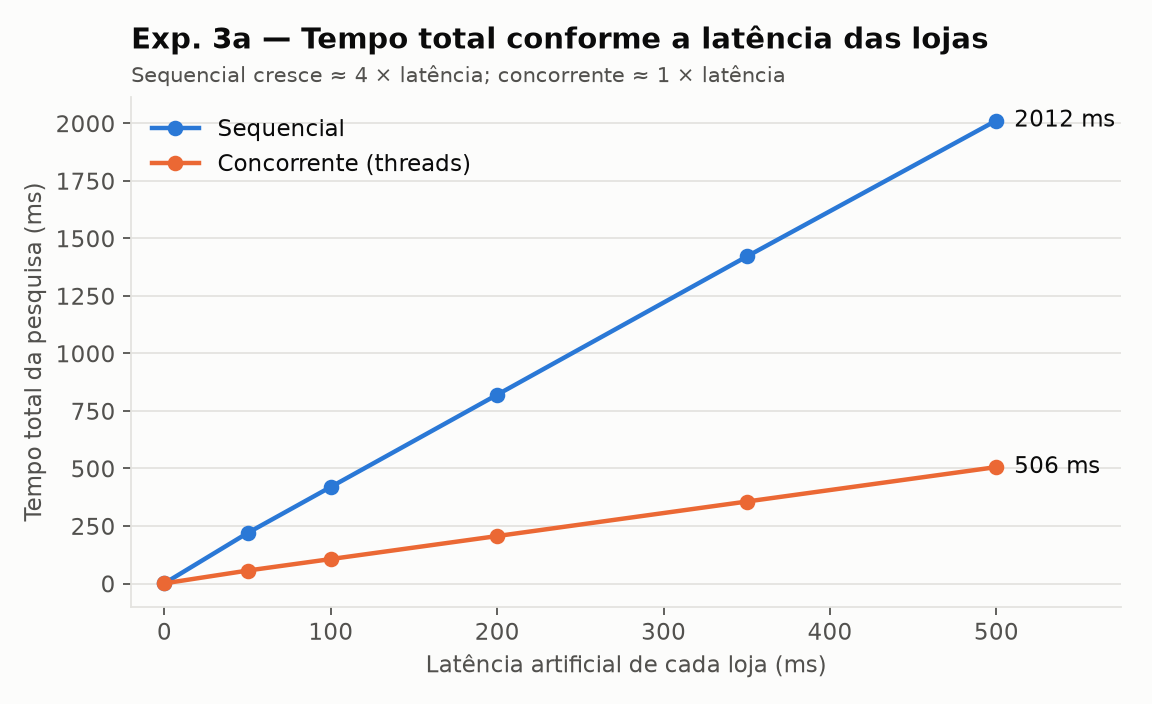
\includegraphics[width=0.78\textwidth]{g2_latencia_uniforme.png}
  \fonteexperimentos
\end{figure}

\FloatBarrier
\subsection{Latências diferentes: 100/200/300/400~ms (3b)}

Na \autoref{tab:exp3b} e na \autoref{fig:g3}, cada loja tem uma latência diferente; a coluna ``Previsto'' é a soma (sequencial) ou o máximo (concorrente) das latências.

\begin{table}[!htbp]
  \centering\small
  \caption{Lojas com latências diferentes (10 repetições)}\label{tab:exp3b}
  \begin{tabular}{@{}lrrrl@{}}
    \toprule
    \textbf{Modo} & \textbf{Média (ms)} & \textbf{Desvio (ms)} & \textbf{Previsto (ms)} & \textbf{Regra} \\
    \midrule
    Sequencial  & 1.020,55 & 3,77 & 1.000 & soma das latências \\
    Concorrente &   405,93 & 1,36 &   400 & maior latência \\
    \bottomrule
  \end{tabular}
  \fonteexperimentos
\end{table}

\begin{figure}[!htbp]
  \centering
  \caption{Lojas com latências heterogêneas (Exp.~3b)}\label{fig:g3}
  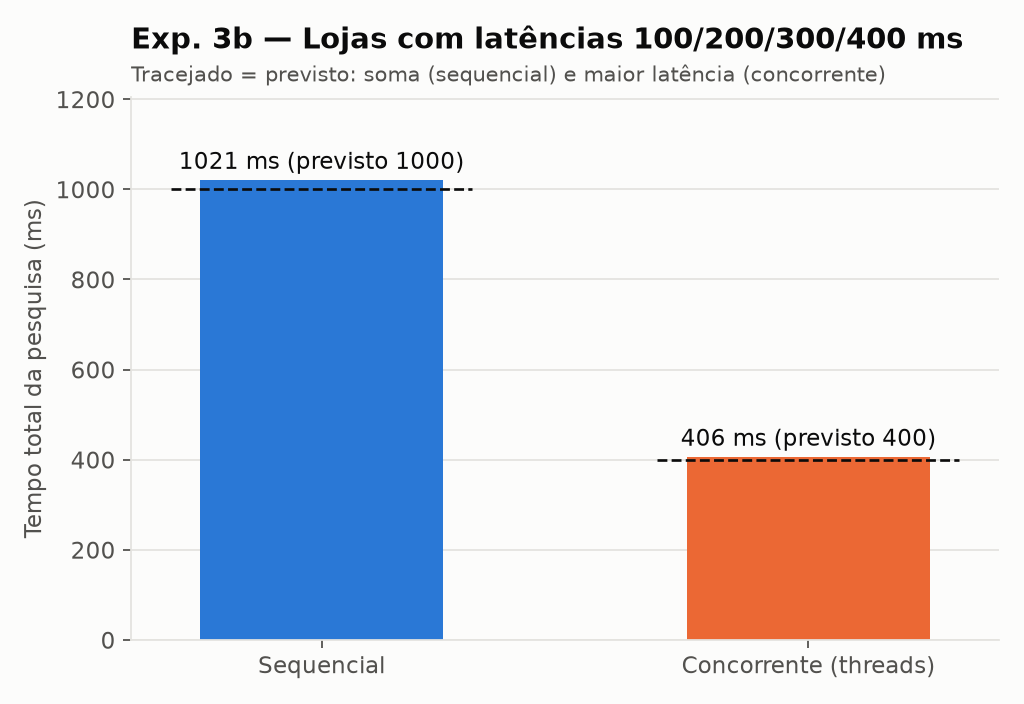
\includegraphics[width=0.78\textwidth]{g3_latencia_heterogenea.png}
  \fonteexperimentos
\end{figure}

\section{Experimento 4 -- múltiplos clientes}

Na \autoref{tab:exp4}, o tempo de resposta é medido no cliente; ``lote'' é o tempo até o último cliente receber a resposta. A \autoref{fig:g4} mostra o tempo de resposta e a \autoref{fig:g5}, a vazão.

\begin{table}[!htbp]
  \centering\small
  \caption{Clientes simultâneos, lojas com 100~ms}\label{tab:exp4}
  \begin{tabular}{@{}rlrrrrr@{}}
    \toprule
    \textbf{Clientes} & \textbf{Modo} & \textbf{Média (ms)} & \textbf{p95 (ms)} & \textbf{Lote (ms)} & \textbf{Vazão (req/s)} & \textbf{Falhas} \\
    \midrule
     1 & sequencial  & 423,07 & 424,33 & 423,27 &   2,36 & 0 \\
     1 & concorrente & 107,39 & 107,59 & 107,55 &   9,30 & 0 \\
     5 & sequencial  & 424,31 & 425,80 & 426,07 &  11,74 & 0 \\
     5 & concorrente & 110,23 & 111,25 & 111,11 &  45,00 & 0 \\
    10 & sequencial  & 425,69 & 428,36 & 427,70 &  23,38 & 0 \\
    10 & concorrente & 111,70 & 112,63 & 113,28 &  88,28 & 0 \\
    20 & sequencial  & 426,08 & 428,80 & 429,27 &  46,59 & 0 \\
    20 & concorrente & 114,59 & 117,77 & 118,39 & 168,93 & 0 \\
    50 & sequencial  & 431,34 & 435,76 & 438,25 & 114,09 & 0 \\
    50 & concorrente & 122,57 & 132,09 & 134,57 & 371,56 & 0 \\
    \bottomrule
  \end{tabular}
  \fonteexperimentos
\end{table}

\begin{figure}[!htbp]
  \centering
  \caption{Tempo de resposta com clientes simultâneos (Exp.~4)}\label{fig:g4}
  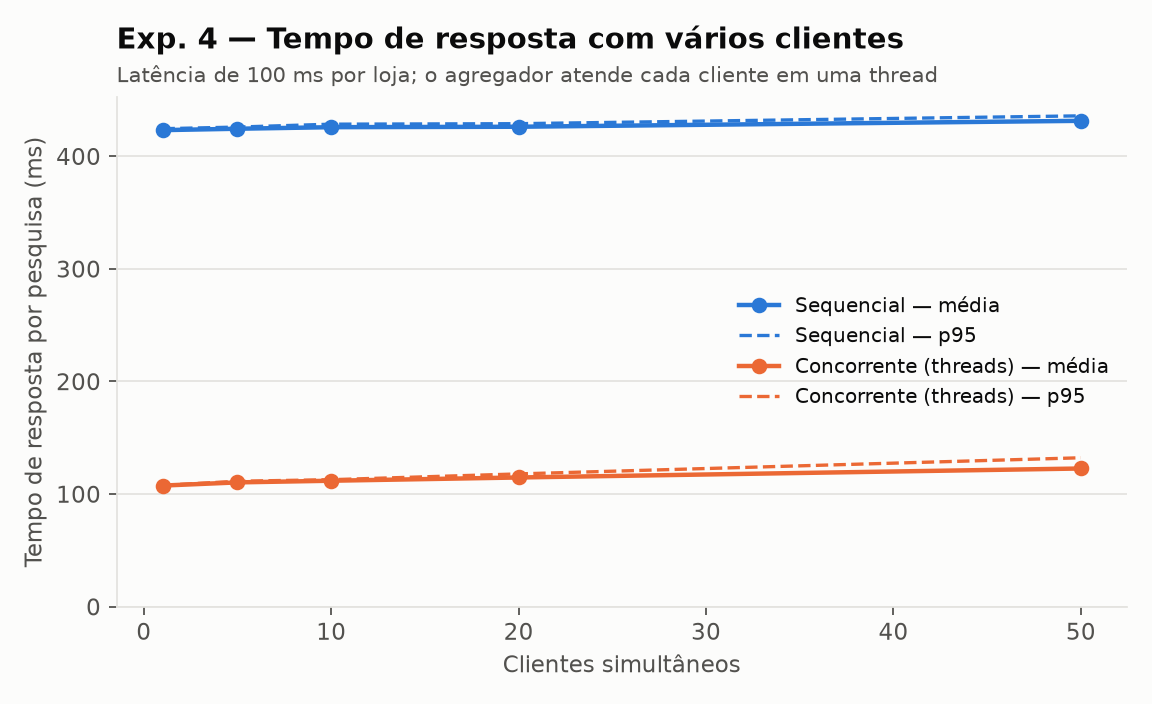
\includegraphics[width=0.78\textwidth]{g4_multiplos_clientes_latencia.png}
  \fonteexperimentos
\end{figure}

\begin{figure}[!htbp]
  \centering
  \caption{Vazão com clientes simultâneos (Exp.~4)}\label{fig:g5}
  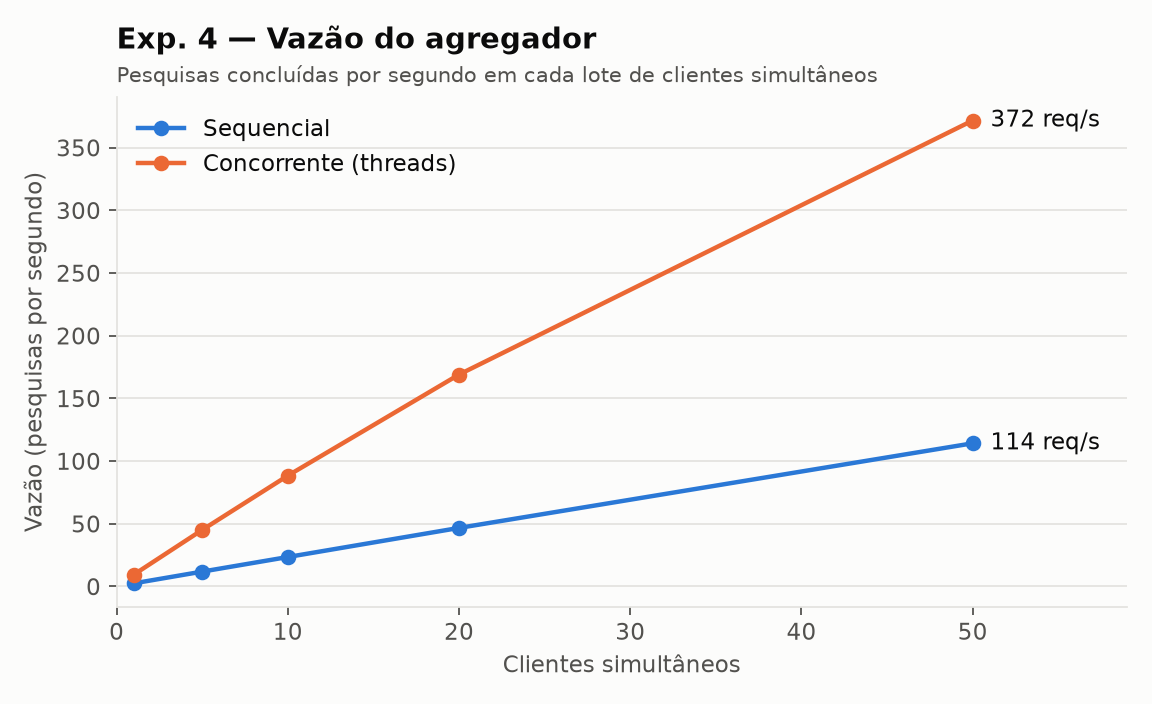
\includegraphics[width=0.78\textwidth]{g5_multiplos_clientes_vazao.png}
  \fonteexperimentos
\end{figure}

\section{Experimento 5 -- indisponibilidade de serviço}

A loja afetada é a MagaluTechSim. Em todos os cenários da \autoref{tab:exp5} a pesquisa foi concluída e o menor preço (PichauSim) foi identificado corretamente; a \autoref{fig:g6} compara os tempos.

\begin{table}[!htbp]
  \centering\footnotesize\setlength{\tabcolsep}{4pt}
  \caption{Indisponibilidade da MagaluTechSim (status e causa referem-se a essa loja)}\label{tab:exp5}
  \begin{tabular}{@{}llrcll@{}}
    \toprule
    \textbf{Cenário} & \textbf{Modo} & \textbf{Tempo (ms)} & \textbf{Lojas OK} & \textbf{Status} & \textbf{Causa} \\
    \midrule
    0) todas ativas        & sequencial  &   618,95 & 4/4 & \cod{sucesso}           & -- \\
    0) todas ativas        & concorrente &   156,23 & 4/4 & \cod{sucesso}           & -- \\
    a) desligada antes     & sequencial  &   465,06 & 3/4 & \cod{erro\_comunicacao} & \cod{ConnectionRefusedError} \\
    a) desligada antes     & concorrente &   156,59 & 3/4 & \cod{erro\_comunicacao} & \cod{ConnectionRefusedError} \\
    b) derrubada durante   & concorrente &   307,69 & 3/4 & \cod{erro\_comunicacao} & \cod{ConexaoEncerrada} \\
    b) derrubada durante   & sequencial  &   757,82 & 3/4 & \cod{erro\_comunicacao} & \cod{ConexaoEncerrada} \\
    c) lenta (timeout)     & sequencial  & 2.964,30 & 3/4 & \cod{timeout}           & \cod{TimeoutError} \\
    c) lenta (timeout)     & concorrente & 2.502,33 & 3/4 & \cod{timeout}           & \cod{TimeoutError} \\
    d) recuperada          & sequencial  &   623,37 & 4/4 & \cod{sucesso}           & -- \\
    d) recuperada          & concorrente &   156,74 & 4/4 & \cod{sucesso}           & -- \\
    \bottomrule
  \end{tabular}
  \fonteexperimentos
\end{table}

\begin{figure}[!htbp]
  \centering
  \caption{Tempo da pesquisa nos cenários de indisponibilidade (Exp.~5)}\label{fig:g6}
  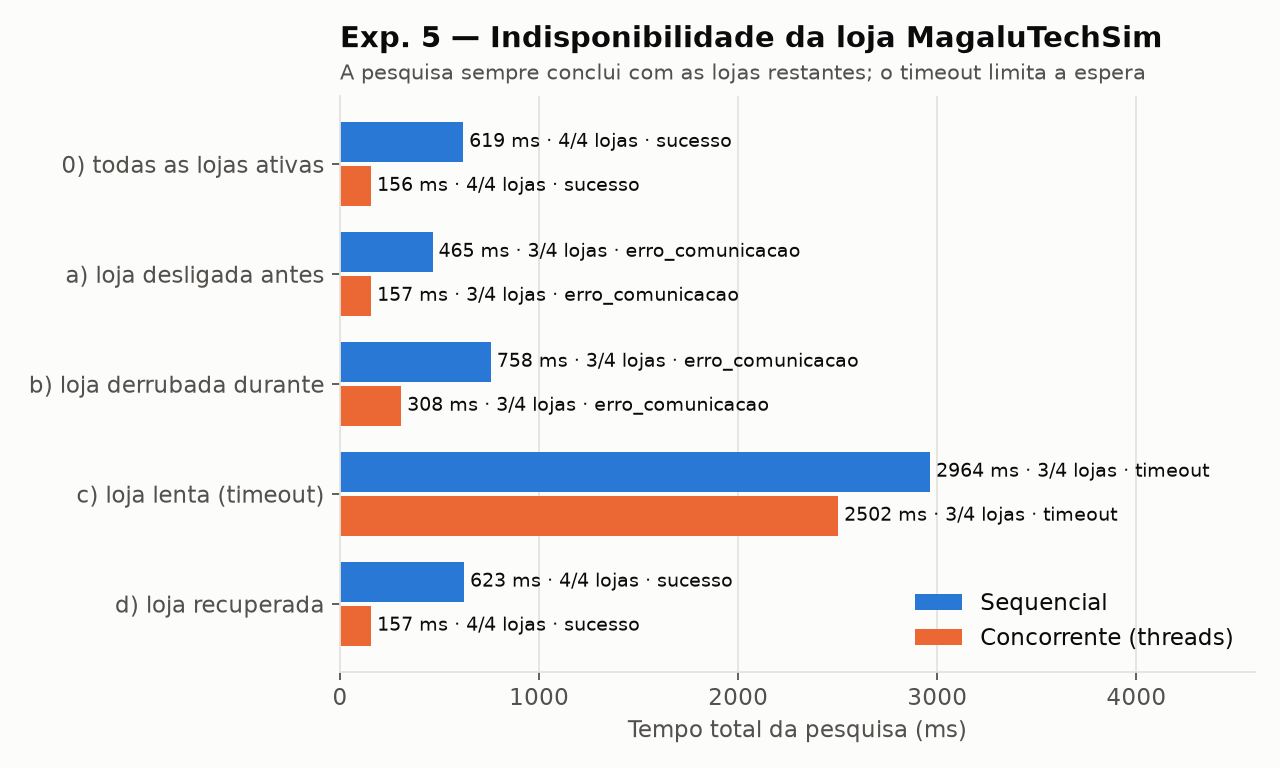
\includegraphics[width=0.78\textwidth]{g6_indisponibilidade.png}
  \fonteexperimentos
\end{figure}

\section{Discussão}

\subsection{Ganho da concorrência (Exp.~1 a 3)}

No modo sequencial, o tempo total segue a soma das latências: 4 × 150~ms = 600~ms previstos contra 621~ms medidos. No modo concorrente, segue a maior latência: 150~ms previstos contra 156,5~ms medidos. O \textit{speedup} observado (3,97) fica praticamente no teórico, igual ao número de lojas (4). O experimento 3b confirma a regra com latências diferentes: o sequencial levou 1.021~ms (soma = 1.000~ms) e o concorrente 406~ms (máximo = 400~ms). O modo concorrente fica limitado pela \textbf{loja mais lenta}, não pelo número de lojas.

\subsection{Por que threads funcionam aqui, mesmo com o GIL}

O trabalho do agregador é quase todo \textbf{espera de entrada e saída}: \cod{connect}, \cod{recv} e a latência das lojas. Durante chamadas bloqueantes de socket e \cod{sleep}, o interpretador Python libera o GIL (\textit{Global Interpreter Lock}), então as quatro esperas se sobrepõem de verdade \cite{python-threading}. Em uma carga limitada por CPU (por exemplo, cálculos pesados no agregador), o GIL serializaria as threads e o ganho praticamente desapareceria; nesse caso seriam necessários processos (\cod{multiprocessing}).

\subsection{Sobrecarga}

Há um custo fixo por consulta: criar o socket, fazer o \textit{handshake} TCP, serializar o JSON e, no modo concorrente, criar a thread. Com latência zero (Exp.~3a), as duas estratégias levam menos de 1~ms e o \textit{speedup} cai para 1,21: quando não há espera, quase não há o que sobrepor. À medida que a latência cresce, a sobrecarga fixa (cerca de 6~ms por pesquisa no modo concorrente e de 5~ms por loja no sequencial) se dilui e o \textit{speedup} tende a 4 (3,90 a 50~ms; 3,98 a 500~ms). Concorrência compensa quando a espera domina o processamento.

\subsection{Múltiplos clientes (Exp.~4)}

O agregador cria uma thread por cliente, por isso clientes simultâneos não esperam uns pelos outros. Mesmo no modo sequencial, o tempo de resposta mudou pouco de 1 para 50 clientes (423 $\rightarrow$ 431~ms). No modo concorrente, com 50 clientes, o agregador manteve cerca de 200 conexões simultâneas com as lojas; o tempo médio subiu só de 107 para 123~ms (p95 = 132~ms) e não houve falhas. A vazão cresceu quase linearmente: de 9,3 para 372~req/s no modo concorrente e de 2,4 para 114~req/s no sequencial.

O pequeno aumento de latência com mais clientes vem da criação de muitas threads e da disputa pelo GIL nos trechos de CPU (\textit{parse} de JSON, ordenação). O modelo de ``uma thread por conexão'' escalaria mal para milhares de clientes (memória por thread, troca de contexto); nesse caso, um \textit{pool} de threads (\cod{ThreadPoolExecutor}) ou entrada e saída assíncrona (\cod{asyncio}) seria mais adequado \cite{tanenbaum2007}.

\subsection{Tolerância a falhas (Exp.~5)}

\begin{itemize}
  \item \textbf{(a) Loja desligada:} a recusa de conexão é detectada em cerca de 1~ms. No modo sequencial a pesquisa até ficou mais rápida (465~ms), porque havia uma loja a menos para esperar.
  \item \textbf{(b) Queda durante a consulta:} o agregador percebeu o fechamento da conexão no momento da queda (308~ms no concorrente, 758~ms no sequencial), sem esperar o timeout.
  \item \textbf{(c) Loja travada:} é o pior caso, e o \textbf{timeout} é essencial. No modo concorrente a espera ficou limitada a cerca de 2,5~s; no sequencial, o timeout soma-se às outras latências (2.964~ms). Sem timeout, a pesquisa ficaria bloqueada indefinidamente.
  \item \textbf{(d) Recuperação:} como cada pesquisa abre conexões novas (protocolo sem estado), a loja recuperada voltou a ser consultada automaticamente, sem reiniciar o agregador.
\end{itemize}

Em todos os casos o resultado parcial (3/4) foi entregue, e a falha foi identificada por loja e por causa.

\subsection{Limitações}

A latência é simulada com \cod{sleep} em \textit{localhost}; uma rede real teria variação (\textit{jitter}) e perdas. Os catálogos são pequenos e estáticos. O agregador não usa cache, nem reenvia consultas que falharam, nem replica as lojas; esses são caminhos naturais para o projeto final da disciplina.

% =================================================================
\chapter{Conclusão}\label{cap:conclusao}

O sistema cumpre os requisitos do enunciado: comunicação real por \textbf{sockets TCP} entre cliente, agregador e \textbf{quatro lojas independentes} (processos separados); consultas \textbf{sequenciais e concorrentes} (threads); atendimento a \textbf{múltiplos clientes}; \textbf{protocolo JSON documentado}; \textbf{tratamento de erros e desconexões}; \textbf{registro do tempo} de cada pesquisa; e consolidação com identificação do menor preço e do melhor custo-benefício. O \autoref{qua:atendimento} relaciona cada requisito técnico da seção~7 do enunciado ao ponto deste relatório que o demonstra.

\begin{quadro}[!htbp]
  \centering\small
  \caption{Atendimento aos requisitos técnicos do enunciado (seção 7)}\label{qua:atendimento}
  \begin{tabularx}{\textwidth}{|L{6.6cm}|Y|}
    \hline
    \textbf{Requisito técnico} & \textbf{Onde é atendido} \\ \hline
    1. Sockets TCP para comunicação entre os componentes & \cod{protocolo.py}, \cod{servidor\_base.py}; \autoref{fig:arquitetura} \\ \hline
    2. Pelo menos quatro serviços independentes & quatro lojas, um processo e uma porta cada (9001--9004) \\ \hline
    3. Consultas sequenciais & \cod{consultar\_todas} (\autoref{cod:consultar-todas}); Exp.~1 \\ \hline
    4. Consultas concorrentes com threads & uma thread por loja + \cod{join()}; Exp.~2 \\ \hline
    5. Atendimento de múltiplos clientes & uma thread por conexão; Exp.~4 (50 clientes, 0 falhas) \\ \hline
    6. Protocolo de aplicação definido e documentado & seção~4.5, \autoref{ap:protocolo} e \cod{docs/03\_protocolo.md} \\ \hline
    7. Tratamento de erros e desconexões & \autoref{qua:falhas}; Exp.~5 \\ \hline
    8. Registro do tempo de execução das pesquisas & \cod{tempo\_total\_ms} e \cod{tempos\_lojas\_ms} em \cod{log\_pesquisas.csv} \\ \hline
    9. Consolidação e apresentação dos resultados & ofertas ordenadas, menor preço e melhor custo-benefício (seção~4.3) \\ \hline
    10. Demonstração durante a apresentação & roteiro do \autoref{qua:roteiro} e interface web \\ \hline
  \end{tabularx}
  \fonteautores
\end{quadro}

Sobre \textit{multithreading}, os experimentos mostram que:

\begin{enumerate}
  \item para consultas independentes e limitadas por entrada e saída, threads reduzem o tempo de resposta da \textbf{soma} para o \textbf{máximo} das latências. Com quatro lojas, o ganho medido foi de 3,97 vezes, praticamente o teórico (4);
  \item o ganho depende de a espera dominar o processamento: com latência nula, o \textit{speedup} é desprezível;
  \item uma thread por cliente permite atender dezenas de usuários simultâneos com aumento pequeno no tempo de resposta e vazão crescendo quase linearmente;
  \item a concorrência também melhora a robustez: uma loja lenta ou fora do ar não atrasa as consultas às demais e, combinada com \textit{timeouts}, garante um limite superior para o tempo da pesquisa.
\end{enumerate}

% ================================================================= PÓS-TEXTUAIS
\postextual
\bibliography{referencias}

% ---------------------------------------------------------------- Apêndices
\begin{apendicesenv}
\partapendices

\chapter{Exemplos de mensagens do protocolo}\label{ap:protocolo}

Este apêndice mostra exemplos das mensagens trocadas pelo protocolo de aplicação. Em cada caso, a mensagem real ocupa uma única linha terminada por \cod{\textbackslash n}; algumas foram quebradas aqui só para caber na página.

\section{Cliente $\rightarrow$ agregador: consultar}

\begin{lstlisting}[style=json]
{"operacao": "consultar", "produto": "rtx 4060",
 "modo": "concorrente", "criterio": "preco"}
\end{lstlisting}

Resposta consolidada (resumida), com a MagaluTechSim fora do ar:

\begin{lstlisting}[style=json]
{"status": "sucesso", "produto_pesquisado": "rtx 4060",
 "modo_execucao": "concorrente", "criterio_ordenacao": "preco",
 "tempo_total_ms": 156.17,
 "tempos_lojas_ms": {"KabumSim": 154.02, "PichauSim": 153.63,
                     "TerabyteSim": 153.74, "MagaluTechSim": 0.8},
 "total_lojas_consultadas": 4, "total_lojas_responderam": 3, "total_ofertas": 3,
 "menor_preco": {...}, "melhor_custo_beneficio": {...},
 "ofertas_ordenadas": [
   {"fonte": "PichauSim", "produto": "GPU Galax GeForce RTX 4060 1-Click OC",
    "specs": "8GB GDDR6, DLSS3, Dual Fan", "preco": 1829.0, "frete": 35.0,
    "preco_total": 1864.0, "avaliacao": 4.7, "garantia_meses": 24,
    "status": "sucesso", "tempo_loja_ms": 153.63,
    "score_custo_beneficio": 14.6951}, ...],
 "lojas_sem_produto": [],
 "ocorrencias_ou_falhas": [
   {"fonte": "MagaluTechSim", "produto": "rtx 4060", "preco": null,
    "preco_total": null, "status": "erro_comunicacao",
    "detalhe": "ConnectionRefusedError: [Errno 61] Connection refused",
    "tempo_loja_ms": 0.8}]}
\end{lstlisting}

\section{Agregador $\rightarrow$ loja: consultar}

\begin{lstlisting}[style=json]
{"operacao": "consultar", "produto": "rtx 4060", "atraso_ms": 150}
\end{lstlisting}

Resposta da loja quando encontra o produto e quando não encontra:

\begin{lstlisting}[style=json]
{"fonte": "KabumSim", "produto": "GPU ASUS Dual RTX 4060 OC 8GB",
 "specs": "8GB GDDR6, DLSS3, 2535MHz", "preco": 1899.9, "frete": 0.0,
 "preco_total": 1899.9, "avaliacao": 4.9, "garantia_meses": 36, "status": "sucesso"}

{"fonte": "KabumSim", "produto": "geladeira", "preco": null, "preco_total": null,
 "status": "nao_encontrado"}
\end{lstlisting}

\section{Listar produtos e ping}

\begin{lstlisting}[style=json]
{"operacao": "listar_produtos"}
-> {"status": "sucesso",
    "produtos": ["iphone", "monitor", "notebook", "rtx 4060", "ssd"],
    "ocorrencias_ou_falhas": []}

{"operacao": "ping"}
-> {"status": "sucesso", "operacao": "pong"}
\end{lstlisting}

\section{Erro de requisição}

\begin{lstlisting}[style=json]
{"operacao": "consultar", "produto": "ssd", "modo": "paralelo"}
-> {"status": "erro_requisicao",
    "detalhe": "modo inválido: 'paralelo'; use ['sequencial', 'concorrente']"}
\end{lstlisting}

\section{Ciclo de vida da conexão}

\begin{lstlisting}[style=json]
cliente                          servidor
   |------ connect() -------------->|   (o servidor cria uma thread para a conexão)
   |------ requisição JSON\n ------>|
   |                                |   processa
   |<----- resposta JSON\n ---------|
   |<----- close() -----------------|   o servidor fecha a conexão após responder
\end{lstlisting}

\end{apendicesenv}

\end{document}
